\documentclass{labreport}
\usepackage{lipsum}
\author{Christoffer Aakre}
\title{Lab Report Class}
\date{11 November 2019}

\begin{document}
\maketitle

The aim of an abstract is to provide a succinct overview of the report.  You have a few lines 
to convince a reader that it is worth the time to look in more detail at your report in order 
to understand how you made your measurements.  You should not only say what it is that 
you have done, but to also highlight any conclusions that are made as the result of any 
work described in this report.  You should be quantitative, so if you measured a quantity,
then you should say what it is.  We measure the speed of light in vacuum to be
$c = (2.99 \pm 0.01) \times \SI{E8}{\meter\per\second}$, which is consistent with the literature.

\section*{Introduction}
The  introduction  to  a  report  is  something  that  you  use  to  help  a  reader  
understand  the  structure  of  what  will  follow.    This  would  be  an  appropriate  place  
in  your  report  for  you  to  put  the  work  into  context  of  the  big  picture.    E.g.  if  you  
are  measuring  the  speed  of  light  –  you  may  choose  to  mention  Special  Relativity,  
and  the  original  historic  tests  of  this  quantity  that  you  are  repeating  in  the  
laboratory.    If  there  are  historical  references,  then  you  could  quote  them  as  Ref.  
[1,2].      Make  sure  that  you  always  use  numbers  to  refer  to  references,  and  that  
the  list  of  references  at  the  end  of  the  report  is  a  numbered  list  (see  below).
It  is  bad  form  to  use  URLs  from  web  sites  as  references.    For  example  Ref.  [3]  
may  change  from  one  day  to  the  next,  and  you  have  no  control  over  the  
authenticity  of  the  material  that  you  are  intending  to  reference.    If  you  want  to
quote  some  source,  then  make  sure  that  you  emphasise  the  text  and  place  it  in  
double  quotes.    For  example  as  George  Leigh  Mallory  noted  \textit{\Quote{Climbers are only a 
particularly foolish set of desperados}}  [4].    One  again  it  is  bad  form  to  copy  long  
quotes  from  other  sources,  hence  avoid  doing  so.    If  you  don’t  cite  the  source,  and  
emphasise  the  text,  then  your  attempt  at  quotation  would  be  plagiarism.

\section*{Background Theory}
The theoretical motivation goes beyond any introduction to include a detailed   
treatise   of   the   problem   at   hand.      Include   equations,   where   necessary   numbering   
them   so   that   you   are   able   to   refer   to   \eqref{eq:mc2}   which   is   Einstein’s   world   famous   
mass energy   relationship:
\begin{equation}
\label{eq:mc2}
    E = mc^2.
\end{equation}
Note   that   punctuation   doesn’t   stop   just   because   you   have   an   equation   in   the   flow   
of   the   text.      A   theory   section   that   does   not   properly   explain   what   it   is   you   are   
trying   to   test,   and   only   relies   on   equations   is   badly   written   and   of   practically   no   
use   to   a   reader.      You   should   make   sure   that   you   provide   enough   of   a   description   
to   help   the   reader   understand   and   encourage   them   to   find   out   why   it   is   that   you   
have   done   what   you   have.      Similarly   writing   that   you   did   this   experiment   
\Quote{because you had to}   has   no   scientific   value   and   therefore   is   inappropriate.

\section*{Experimental setup}
When describing the experimental setup you are using, you should always make 
sure that you include any relevant information in terms of model numbers of 
components, or types of equipment that you are using as your signal generator.  
For example, we used a Keithly 1776 DMM to measure voltage for our circuit.  
This level of information may seem pedantic, however it will give a reader the 
opportunity to recreate your results by performing a repeat experiment under 
circumstances that will be very close to the original.  Similar if your results 
depend on the temperature of the environment make sure that you take note of 
this.  As the saying goes,  \Quote{a picture tells a thousand words}, so it may be necessary 
to refer to Figures in your report.  When you do, refer to them by number, e.g. 
\figref{fig:detector}, and indicate in the text and caption of the Figure what it is that the 
reader should take away with them.

\begin{figure}
    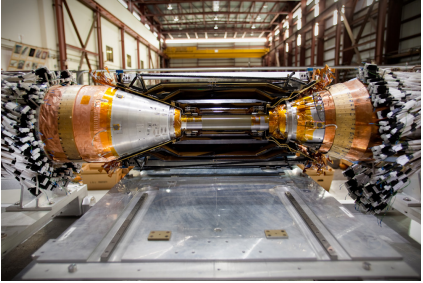
\includegraphics{Capture}
    \caption{A cross-sectional view of the silicon vertex detector from the BaBar 
experiment (See Ref [5]).}
    \label{fig:detector}
\end{figure}

Note that the caption of the figure is written in such a way that usually one does 
not have to refer to the text to understand what this represents.  In some 
complicated circumstances one might depart from this approach and refer to 
equations or other information described in the text.  This is all with an aim of 
helping your reader understand what it is you have done.

\section*{Results and Discussion}
Results should include a description of what it is you have measured.  Where 
appropriate you should refer to Tables by number, and tabulate sets of common 
data.  If for example you measure the length of a component of your experiment 
you can report this as $x=(10.2 \pm 2) \SI{}{\milli\meter}$ long.  Note that a measurement always has 
a value, an error and units.  The units are common both to the value and error, 
unless for some particular reason it is appropriate to quote the error as a 
percentage of the value.  In which case you can say that $x$ has been measured to 
$20\%$.  When quoting errors always consider the appropriate number of 
significant figures required, and refer back to your notes if necessary. \tableref{tab:values}
shows the results of some dummy experiment.

\begin{table}
    \begin{tabular}{c c c}
     \cr & \textbf{Measured value (m)} & \textbf{Error (m)}  \\
    \textbf{Height} & 0.5 & 0.01 \\
    \textbf{Length} & 2.7 & 0.01 \\
    \textbf{Depth} & 3.1 & 0.01 \\
    \end{tabular}
    \caption{Some dummy data to illustrate how to comment about the table, and 
link the table from the text.}
    \label{tab:values}
\end{table}

Having included a table of data, at some point it may become necessary to 
analyse the data, for example by fitting the data.  If that is the case, make sure 
that any figures includes are referenced appropriately with captions, axis labels 
for both the ordinate and abscissa.  You should also consider if it is necessary to 
include error bars on the data.  The interpretation of any model fitted to data 
should then be discussed in the results section.  As an example, \figref{fig:distribution} shows 
the distribution of two populations of data (A and B) that are generated 
according to a uniform Gaussian distribution using ROOT [6].  Note here that the 
reference given for ROOT is a URL as that is appropriate in this particular 
instance.

\begin{figure}
    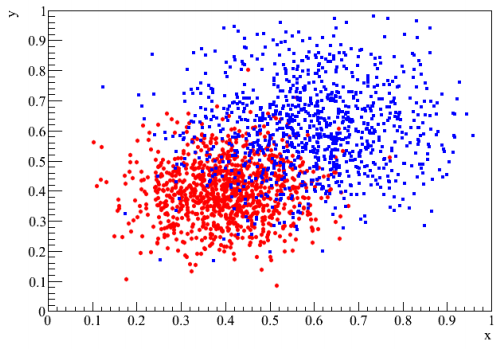
\includegraphics{diagrams/distribution.PNG}
    \caption{Distributions (red) A and (blue) B generated in $x$ and $y$ from random 
Gaussian distributions with different means and widths.  Note that in general it is 
better to use different marker or line styles to refer to different populations of 
data or fit hypotheses, as will become apparent if you choose to print this test 
report off on a black and white printer.}
    \label{fig:distribution}
\end{figure}

One last point that should be made is that in addition to the suggested reading on 
style and report writing, you can find suitable information online.  One 
particularly thorough reference is the American Physical Society (APS) style 
guide [7].  If you are interested in the finer points on how to prepare a report 
with a legitimate scientific style, please take a look at that.

\section*{Conclusions}
Often the second section of an article that is read is a conclusion – so that a 
reader may better understand what it is that you have achieved and for them to 
decide if it is worth the effort in going through the whole article in detail.  You 
should encapsulate a summary of any and all conclusions that you are able to 
make within this section.  As with the abstract, you should be quantitative in 
your conclusions.  We measure the speed of sound in air to be 
$330 \pm 30 \SI{}{\meter\per\second}.$There is no excuse for not running the spell checker on your report. Finally – you 
should refer to the suggested texts on style and preparing a report, and give your 
report a final proof-read before submitting it. 

\printbibliography

\end{document}